% Instructions to change to html version:
% Comment out:
%  minipage, multicols,columnbreak, mathbf, hrule
% Replace all: \begin{minipage}% \end{minipage} %\begin{multicols}  %\end{multicols}  %\columnbreak %% \begin{framed} %\end{framed} %%\hrule
% Replace \mathbf with \boldsymbol
% Replace $$ with \[ or \]and $ with \( or \)
% Enclose graphics in figure environments and add captions
% 			search \includegraphics
% Re-tag \df environments as sections, subsections, etc.
% Command Line Code to Create html version:
%First: pdflatex -shell-escape filename.tex                                   
%Second, for each figure: inkscape "filename-figure1.pdf" -o "filename-figure1.png"
% Third: htlatex filename.tex "ht5mjlatex.cfg, charset=utf-8" " -cunihtf -utf8"

\documentclass[10pt]{article}

%\usepackage{tikz, pgf,pgfplots,wasysym,array}
%\usepackage{wasysym,array}

\usepackage{amsmath,amssymb}

\ifdefined\HCode
  \def\pgfsysdriver{pgfsys-tex4ht-updated.def}
\fi 
%\ifdefined\HCode
%  \def\pgfsysdriver{pgfsys-dvisvgm4ht.def}
%\fi 
\usepackage{tikz}
\usetikzlibrary{calc,decorations.markings,arrows}
\usepackage{pgfplots}

\pgfplotsset{compat=1.12}
\usepackage{myexternalize}
\usetikzlibrary{calc,decorations.markings,arrows}
\usepackage{framed}
\usepackage[none]{hyphenat}

\input{../../../common/1336_header_test.tex}
\begin{document}

\everymath{\displaystyle}


\newcommand{\ihat}{\boldsymbol{\hat{\textbf{\i}}}}
\newcommand{\jhat}{\boldsymbol{\hat{\textbf{\j}}}}
\newcommand{\khat}{\boldsymbol{\hat{\textbf{k}}}}

\let\oldvec\vec
\renewcommand{\vec}[1]{\oldvec{\boldsymbol{#1}}}

\renewcommand{\u}{\vec{u}}
\renewcommand{\v}{\vec{v}}
\newcommand{\w}{\vec{w}}
\renewcommand{\r}{\vec{r}}
\renewcommand{\a}{\vec{a}}
\renewcommand{\b}{\vec{b}}
\renewcommand{\c}{\vec{c}}

\newcommand{\<}{\left\langle}
\renewcommand{\>}{\right\rangle}

\renewcommand{\myTitle}{MATH 1336: Calculus III}

\renewcommand{\mySubTitle}{Section 2.4: Cross Product \vspace*{-.2in}}
%~\hfill Name: \underline{~~~~~~~~~~~~~~~~~~~~~~~~~~~~~~~~~~~~~~~~~~~~~~~}

\lectTitle{\vspace*{-.5in}\myTitle}{\vspace*{.1in}\mySubTitle \vspace*{-.1in}}


\setlength{\columnseprule}{0.4pt}
\setlength{\columnsep}{3em}

%\hspace*{-.8in}%\begin{minipage}{1.25\textwidth}
%\begin{framed}


\section*{Cross Product Definition:}
\vspace*{-.2in}
%\begin{multicols}{2}
The \textbf{cross product} of two vectors, \(\vec{a}=\<a_1,a_2,a_3\>, \b=\<b_1,b_2,b_3\>\) results in a vector that is orthogonal to both \(\a\) and \(\b\). \\~\\

\[
\a \times \b = \begin{array}{|ccc|}
~\ihat & \jhat & \khat~\\
a_1 & a_2 & a_3\\
b_1 & b_2 & b_3
\end{array}
 = \left|\begin{array}{cc}
 a_2 & a_3\\
 b_2 & b_3
 \end{array}
 \right|
 \ihat
 - \begin{vmatrix}
 a_1 & a_3\\
 b_1 & b_3
 \end{vmatrix}
 \jhat
 + \begin{vmatrix}
 a_1 & a_2\\
 b_1 & b_2
 \end{vmatrix}
 \khat
 = \left(a_2 b_3 - a_3 b_2\right) \ihat - \left( a_1 b_3 - a_3 b_1\right) \jhat + \left( a_1 b_2 - a_2 b_1\right) \khat
\]

~\\

The direction of the vector \(\a \times \b\) is determined using the \textbf{right hand rule}, and it's magnitude is given by \(||\a \times \b|| = ||\a||\ ||\b|| \sin\theta\), where  \(\theta\) is the angle between \(\a\) and \(\b\).\\


 

%\columnbreak
%
%\end{multicols}

%\hrule
\vspace*{.1in}
\subsection*{Right Hand Rule:}



\begin{figure}[!h]
\centering
\includegraphics[height=1in]{Ch2s4-right-hand-rule.png}
\caption{Figure used to demonstrate the right hand rule.}
\end{figure}

%\end{minipage}
\hspace*{.2in}
%\begin{minipage}{.5\textwidth}

To determine the direction of \(\a \times \b\), point the fingers of your \textit{right hand} in the direction of \(\a\), then curl them toward \(\b\). Your thumb will then point in the direction of \(\a \times \b\)!\\

Note that order matters! (See property 1 on the next page.)\\

%\end{minipage}

%\hrule
%\vspace*{.1in}
%\df{\textcolor{sblack}{Algebraic Properties of the Cross Product:}}~\\
%
%
%\(\a, \b, \c\) are all vectors in either \(\mathbb{R}^2\) or \(\mathbb{R}^3\), and \(s\) is a scalar 
%\begin{enumerate}
%\item \(\a \times \b = -\ \b \times \a\)
%\item \((s\a) \times \b =s(\a \times \b) = \a \times (s\b)\)
%\item \(\a \times \left(\b +\c\right) = \a \times \b + \a \times \c\)
%\item \(\left(\a +\b\right) \times \c = \a \times \c + \b \times \c\)
%\item \( \a \cdot \left(\b \times \c\right) = \left( \a \times \b\right) \cdot \c\)
%\item \( \a \times \left(\b \times \c\right) = \left( \a \cdot \c\right) \b - \left(\a  \cdot \b\right) \c\)
%\end{enumerate}
%
%%\hrule
%%\vspace*{.1in}

%\end{framed}
%\end{minipage}

\section*{Example 1:} %(Pre-class Video):} 

Find \(\a \times \b\) and verify that it is perpendicular to \(\a\) and \(\b\).
\[ \a = \<1, 2, 3\>, \qquad \b = \<4, 5, 6\> \]



\[
\a \times \b = \begin{vmatrix}
\ihat & \jhat & \khat\\
1 & 2 & 3\\
4 & 5 & 6
\end{vmatrix}
 = \begin{vmatrix}
 2 & 3\\
 5 & 6
 \end{vmatrix}
 \ihat
 - \begin{vmatrix}
 1 & 3\\
 4 & 6
 \end{vmatrix}
 \jhat
 + \begin{vmatrix}
 1 & 2\\
 4 & 5
 \end{vmatrix}
 \khat
 = \left[(2) (6) - (3)( 5)\right] \ihat - \left[ (1) (6) - (3)( 4)\right] \jhat + \left[ (1)( 5) - (2) (4)\right] \khat
\]

\[
\a \times \b = \left(12 - 15\right) \ihat - \left( 6 - 12 \right) \jhat + \left( 5 - 8 \right) \khat = \<-3, 6, -3\>
\]

\vfill

To verify that the result is perpendicular to both \(\a\) and \(\b\), use the dot product!

\[
\left(\a \times \b\right) \cdot \a = \<-3, 6, -3\> \cdot \<1, 2, 3\> = -3 + 12 -9 = 0
\]

\[
\left(\a \times \b\right) \cdot \b = \<-3, 6, -3\> \cdot \<4, 5, 6\> = -12+30-18 = 0
\]

\vfill

\pagebreak

%\hspace*{-.8in}%\begin{minipage}{1.25\textwidth}
%\begin{framed}

\section*{Algebraic Properties of the Cross Product:}


\(\a, \b, \c\) are all vectors in either \(\mathbb{R}^2\) or \(\mathbb{R}^3\), and \(s\) is a scalar 
\begin{enumerate}
\item \(\a \times \b = -\ \b \times \a\)
\item \((s\a) \times \b =s(\a \times \b) = \a \times (s\b)\)
\item \(\a \times \left(\b +\c\right) = \a \times \b + \a \times \c\)
\item \(\left(\a +\b\right) \times \c = \a \times \c + \b \times \c\)
\item \( \a \cdot \left(\b \times \c\right) = \left( \a \times \b\right) \cdot \c\)
\item \( \a \times \left(\b \times \c\right) = \left( \a \cdot \c\right) \b - \left(\a  \cdot \b\right) \c\)
\end{enumerate}

%\hrule
\vspace*{.1in}

\section*{Geometric Properties of the Cross Product:}





\begin{figure}[!h]
\centering
\includegraphics[height=1.5in]{Ch2s4-area-parallelogram.png}
\caption{Diagram illustrating the area of a parallelogram determined by vectors a and b.}
\end{figure}

\hspace*{.2in}
%\begin{minipage}{.5\textwidth}

 The area of the parallelogram determined by \(\a\) and \(\b\) is given by
 \[A_{\text{parallelogram}} =||\a \times \b|| =||\a||\ ||\b|| \sin\theta\]

The area of the triangle \(PQR\) is half of the area of the parallelogram:
 \[A_{\text{triangle}} = \frac{1}{2}||\a \times \b||\]
 
 These areas would be zero if the vectors were parallel:\\

 Vectors \(\a\) and \(\b\) are parallel if-and-only-if \(\a \times \b = \vec{0}\).\\

%\vspace*{-.2in}
%\end{minipage}

%\hrule
\vspace*{.1in}



\section*{Torque: }

\begin{figure}[!h]
\centering
\includegraphics[height=2in]{Ch2s4-torque3.png}
\caption{Diagram illustrating applied torque using a ratchet on a bolt under Dr. Cole's desk.}
\end{figure}


%\end{minipage}
\hspace*{.2in}
%\begin{minipage}{.5\textwidth}

The \textbf{torque}, \(\vec{\tau}\), from applying a force \(\vec{F}\) to a rigid body at a point given by position vector \(\vec{r}\) is  calculated using:

\begin{align*}
\vec{\tau} &= \vec{r} \times \vec{F} \\
||\vec{\tau}|| &= ||\vec{r}||\ ||\vec{F}|| \sin\theta
\end{align*}

\[ ||\vec{\tau}|| = (\text{length of wrench})*(\text{component of force perpendicular to wrench}) \]

~\\

 ``righty-tighty, lefty-loosy" rule \(\Leftrightarrow\) right hand rule for cross products!

\vspace*{.5in}

%\end{minipage}


%\end{framed}
%\end{minipage}

%%\begin{framed}
%\textbf{Vocabulary \& Definitions:} \\~\\
%The \textbf{cross product} of two vectors, \(\vec{a}=\<a_1,a_2,a_3\>, \b=\<b_1,b_2,b_3\>\) results in a vector that is orthogonal to both \(\a\) and \(\b\). 
%\[
%\a \times \b = \begin{vmatrix}
%\ihat & \jhat & \khat\\
%a_1 & a_2 & a_3\\
%b_1 & b_2 & b_3
%\end{vmatrix}
% = \begin{vmatrix}
% a_2 & a_3\\
% b_2 & b_3
% \end{vmatrix}
% \ihat
% - \begin{vmatrix}
% a_1 & a_3\\
% b_1 & b_3
% \end{vmatrix}
% \jhat
% + \begin{vmatrix}
% a_1 & a_2\\
% b_1 & b_2
% \end{vmatrix}
% \khat
%\]
%
%The direction of the vector \(\a \times \b\) is determined using the \textbf{right hand rule}, and it's magnitude is given by \(|\a \times \b| = |\a| |\b| \sin\theta\), where  \(\theta\) is the angle between \(\a\) and \(\b\).\\
%
% The area of the parallelogram determined by \(\a\) and \(\b\) is given by \(|\a \times \b| = |\a| |\b| \sin\theta\)\\
% 
% Vectors \(\a\) and \(\b\) are parallel if-and-only-if \(\a \times \b = \vec{0}\).
%
%%\end{framed}
%
%\section*{Torque:}
%\includegraphics[width=\textwidth]{Ch10s4-torque.pdf}


\section*{Vector Problems for Group Work:}

\newcounter{prob}

\begin{list}{\bf{Problem \arabic {prob}: }}{\usecounter{prob}}

\item  Evaluate the following cross products.  Do the results agree with your intuition?

\begin{enumerate}[a)]

\item \(\ihat \times \jhat\)

%\vspace*{.25in}
\vfill

\item \(\jhat \times \khat\)

%\vspace*{.25in}
\vfill

\item \(\left\langle 1, 1, 0\right\rangle \times \left\langle -1, 1, 0\right\rangle\)

%\vspace*{.25in}
\vfill

\end{enumerate}


\item Compute the area of the triangle determined by \(\vec{a} = \left\langle 1, -2, 6\right\rangle\) and \(\vec{b} = \left\langle 4, 3, -1\right\rangle\).

\vfill

%\pagebreak


\item  Let \(\vec{a} = s\vec{b}+t\vec{c}\), where \(s\) and \(t\) are scalars.
  Show that \(\vec{a}\cdot (\vec{b} \times \vec{c}) = 0\).

\vfill

%\pagebreak

\item \textbf{Vector, Scalar, or Nonsense?}\\Some of the expressions below are meaningful, and some are not.  Determine which expressions make sense, and if the result is a scalar or a vector:

%\begin{multicols}{2}
\begin{enumerate}[a)]

\item \(\vec{a} \cdot (\vec{b} \times \vec{c})\)
\vspace*{.25in}

\item \(\vec{a} \times (\vec{b} \cdot \vec{c})\)
\vspace*{.25in}

\item \(\vec{a} \times (\vec{b} \times \vec{c})\)
\vspace*{.25in}

\item \(\vec{a} \cdot (\vec{b} \cdot \vec{c})\)
\vspace*{.25in}

\item \((\vec{a} \cdot \vec{b}) \times (\vec{c} \cdot \vec{d})\)
\vspace*{.25in}

\item \((\vec{a} \times \vec{b}) \cdot (\vec{c} \times \vec{d})\)
\vspace*{.25in}

\end{enumerate}
%\end{multicols}

\item  \textbf{(Fun Geometry Challenge!)}\\
 Use vector methods to show that any angle inscribed on a semicircle is a right angle.\\
 \label{geom-challenge}.
 
%\textit{Hint:} Impose a coordinate system on the figure below, with the origin located at the center of the circle, which is marked \(0\). Find the coordinates of the point \(P\) in terms of \(\theta\).
  
\begin{figure}[!h]
\centering
\hspace*{-.75in}
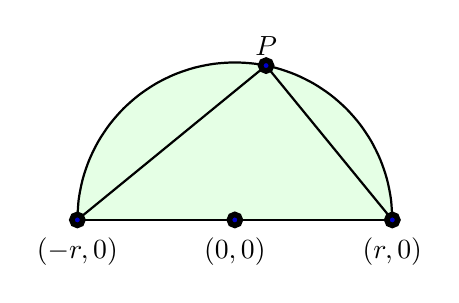
\begin{tikzpicture}
\begin{axis}[
	y=1cm,
    x=1cm,
	axis x line=none,
	axis y line = none,
	ymin=-.7,ymax=3,
	xmin=-3,xmax = 3,
    grid=none
     %xticklabels={\(-\pi\), \( \), ,\( \),\(\pi\)},
%    xtick={-3.14,-1.57,...,3.14},
%    ytick={0,.25,...,1.25},
%    xlabel=\(x\),
%    ylabel=\(y\),
%    tick label style={font=\footnotesize},
]



\addplot[thick,black, fill=green!20,fill opacity = .5, domain=0:180, smooth] ({2*cos(x)},{2*sin(x)});

\addplot[thick,black, domain=-2:2 ] {0};
\addplot[thick,black, domain=-2:.397 ] {.818*(x+2)};
\addplot[thick,black, domain=.397:2 ] {-1.222*(x-2)};
\addplot+[black,only marks, mark=*, line width=2pt] coordinates{(.397,1.960)(-2,0)(2,0)(0,0)};
\node [above] at (axis cs:  .397,1.960) {\(P\)};
\node [below] at (axis cs:  0,-.1) {\((0,0)\)};
\node [below] at (axis cs:  2,-.1) {\((r,0)\)};
\node [below] at (axis cs:  -2,-.1) {\((-r,0)\)};

\end{axis}
\end{tikzpicture}
\caption{Diagram for Problem \ref{geom-challenge}.}
\end{figure}

%\vspace*{1in}

\end{list}

\end{document}
